\documentclass[a4paper,12pt]{article}
\usepackage[utf8]{inputenc}
\usepackage{graphicx}
\usepackage[margin=1in]{geometry}
\usepackage{titling}
\usepackage{fancyhdr} % header and footer
\usepackage{everypage}
\usepackage{hyperref}
\usepackage{array}
\graphicspath{ {./images} }

\hypersetup{
    colorlinks=false,
}

\fancypagestyle{plain}{ 
    \fancyhf{}
    \renewcommand{\headrulewidth}{0pt}
    \renewcommand{\footrulewidth}{0pt}
}

\fancyhf{}
\fancyhead[L]{
\includegraphics[width=0.3\textwidth]{logo_ipl.png}}
\fancyhead[R]{
    \small Licenciatura em Eng. Informática\\
    Ano Letivo 2024/2025\\
    Sistemas Gráficos e Interação -- Projeto
}
\setlength{\headsep}{2cm}
\renewcommand{\headrulewidth}{0pt}
\renewcommand{\contentsname}{Índice}

\fancyfoot[R]{\thepage} 
\setlength{\footskip}{0cm}
\pagestyle{fancy}

\begin{document}

\begin{titlepage}
\begin{center}
    
\includegraphics[width=0.5\textwidth]{logo_ipl.png}
\end{center}

\vspace{1cm}

\begin{center}
    \fboxsep=10pt
    \parbox[c][3cm][c]{0.8\textwidth}{
        \centering
        \textbf{\Large Relatório do Projeto de}\\[0.3cm]
        \textbf{\Large Interface web 3D}
    }
\end{center}

\vfill

\begin{center}
    \textbf{Licenciatura em Engenharia Informática}\\
    Sistemas Gráficos e Interação\\[0.5cm]
    \vspace{1cm}
    \textbf{Ano Letivo: 2024/2025}
\end{center}

\vfill

% Student information
\begin{center}
    \textbf{Estudantes:}\\[0.3cm]
    Marco Padeiro, 2231953\\
    Rodrigo Carreira, 2231952
\end{center}
\thispagestyle{plain}
\end{titlepage}

\newpage
\tableofcontents

\newpage
\section{Avaliação heurística}

\begin{center}

\begin{table}[h!]
    \centering
    \begin{tabular}{|m{3cm}|m{12cm}|}
    \hline
    \multicolumn{2}{|c|}{\textbf{Registo 1}} \\ \hline
    \textbf{Tarefa}       & Acesso a página de Login/Registo \\ \hline
    \textbf{Local}        & Ao abrir a página de Login/Registo \\ \hline
    \textbf{Heurística}   & 4 \\ \hline
    \textbf{Descrição}    & O footer presente nesta página não se encontra no fundo da página. \\ \hline
    \textbf{Frequência}   & Apenas uma vez \\ \hline
    \textbf{Persistência} & Persistente \\ \hline
    \textbf{Severidade}   & 1 \\ \hline
    \textbf{Solução}      & Fazer com que o footer fique no fundo da página mesmo que está não tenha conteudo sufiente para preencher uma página completa. \\ \hline
    \end{tabular}
\end{table}

\vspace{0.5cm}
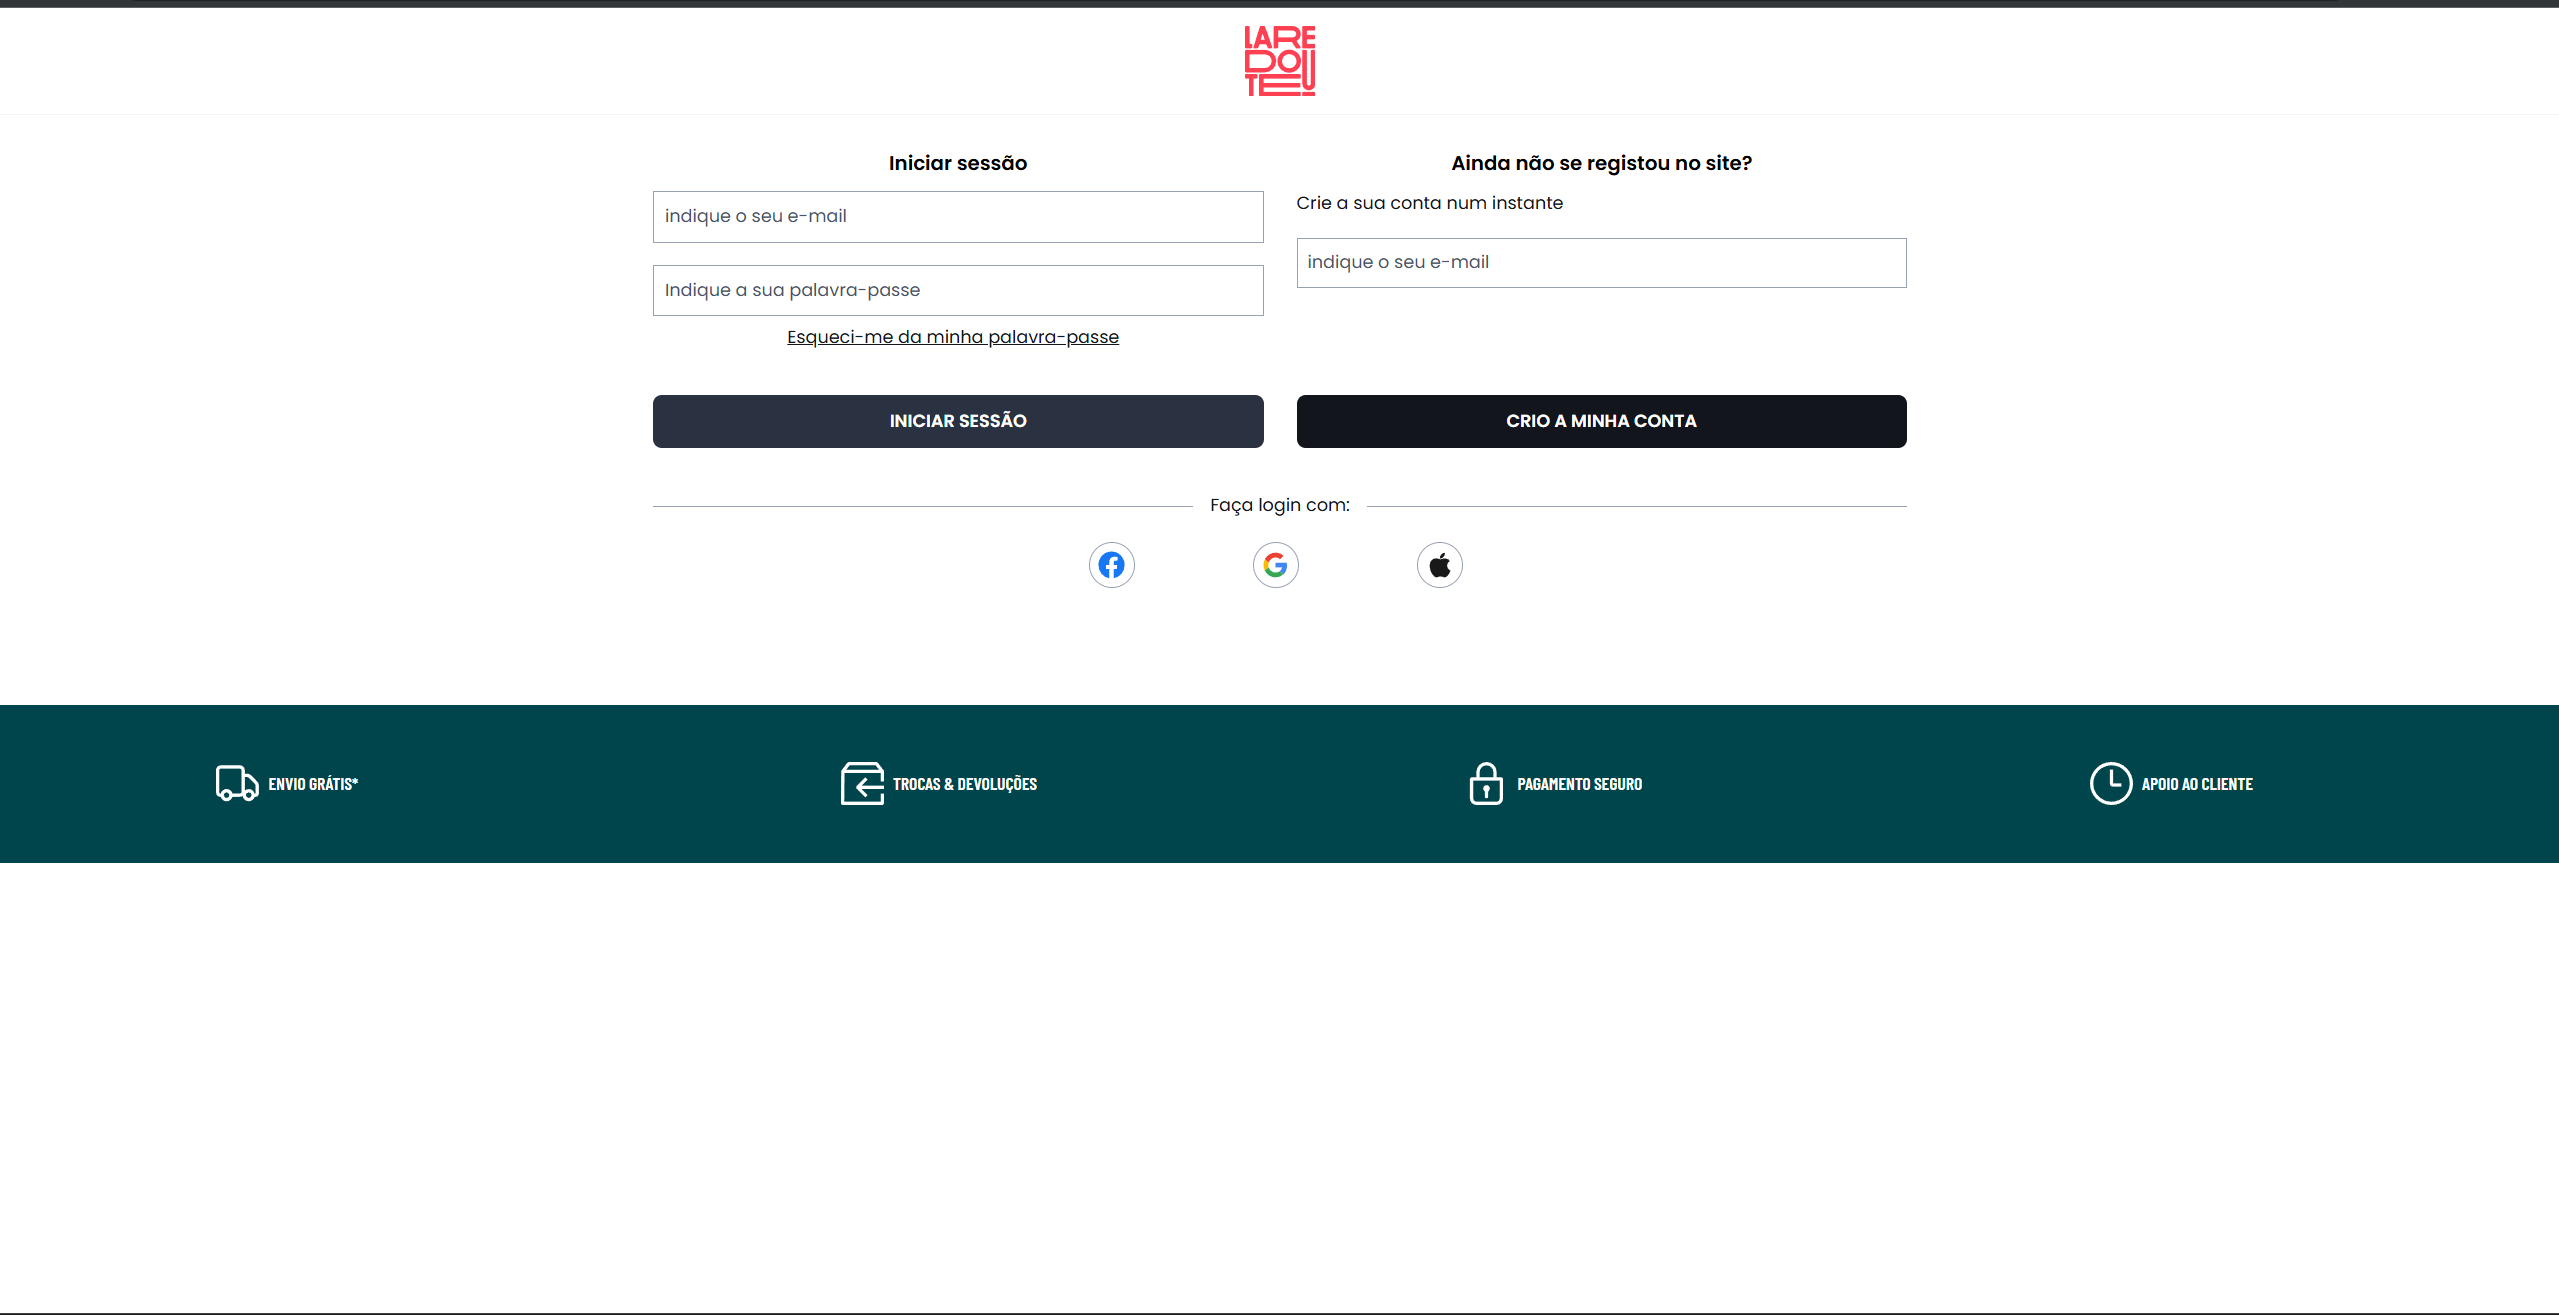
\includegraphics[width=\textwidth, keepaspectratio]{heuristics/01footer_registo.png}
    

\newpage
    \begin{table}[h!]
        \centering
        \begin{tabular}{|m{3cm}|m{12cm}|}
        \hline
        \multicolumn{2}{|c|}{\textbf{Registo 2}} \\ \hline
        \textbf{Tarefa}       & Visualizar detalhes do produto. \\ \hline
        \textbf{Local}        & Ao editar a quantidade pretendida de um produto. \\ \hline
        \textbf{Heurística}   & 4, 8 \\ \hline
        \textbf{Descrição}    & A utilização de um input numérico com botões de '+' e '-' é mais intuitiva e dinâmico do que o uso de um input do tipo select. \\ \hline
        \textbf{Frequência}   & Sempre \\ \hline
        \textbf{Persistência} & Persistente \\ \hline
        \textbf{Severidade}   & 0 \\ \hline
        \textbf{Solução}      & Utilizar um input numérico com limite variável conforme o produto e botões de incremento.\\ \hline
        \end{tabular}
    \end{table}
    
    \vspace{0.5cm}
    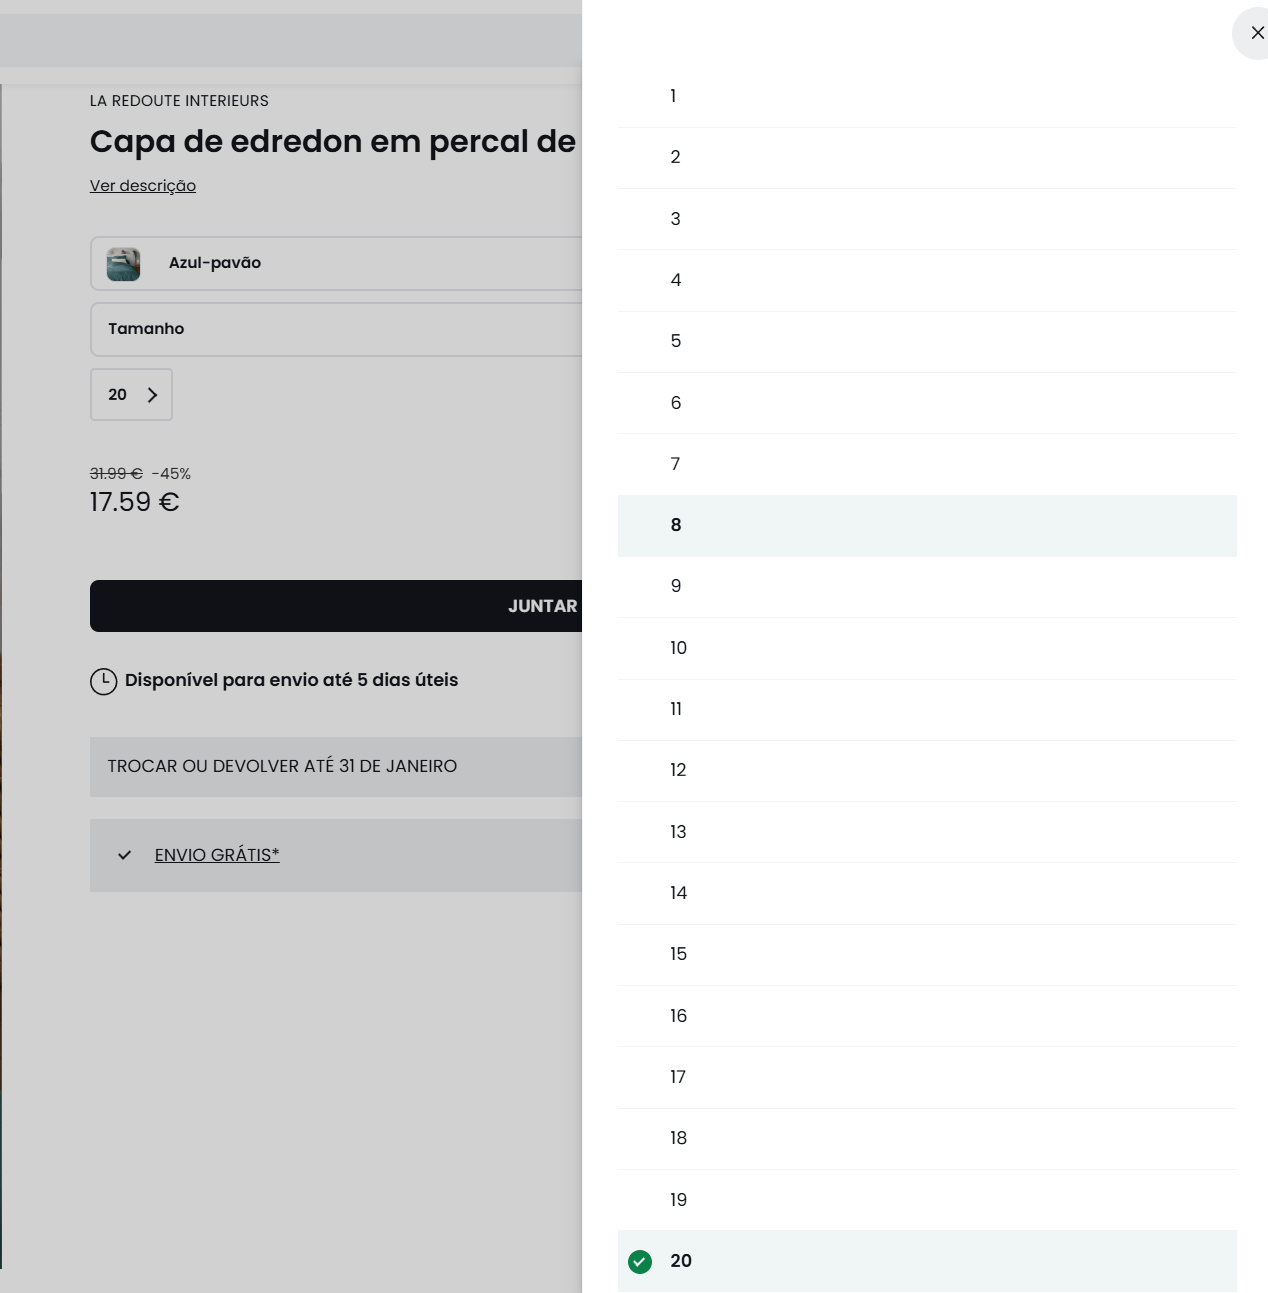
\includegraphics[width=\textwidth, keepaspectratio]{heuristics/02input_quantidade.png}

\newpage
    \begin{table}[h!]
        \centering
        \begin{tabular}{|m{3cm}|m{12cm}|}
        \hline
        \multicolumn{2}{|c|}{\textbf{Registo 3}} \\ \hline
        \textbf{Tarefa}       & Acedar ao carrinho \\ \hline
        \textbf{Local}        & Página de carrinho \\ \hline
        \textbf{Heurística}   & 4  \\ \hline
        \textbf{Descrição}    & Os breadcrumbs estão muito próximos da margem da página. \\ \hline
        \textbf{Frequência}   & Sempre \\ \hline
        \textbf{Persistência} & Persistente \\ \hline
        \textbf{Severidade}   & 1 \\ \hline
        \textbf{Solução}      & Adicionar uma margem entre o início da página e os breadcrumbs. \\ \hline
        \end{tabular}
    \end{table}
    
    \vspace{0.5cm}
    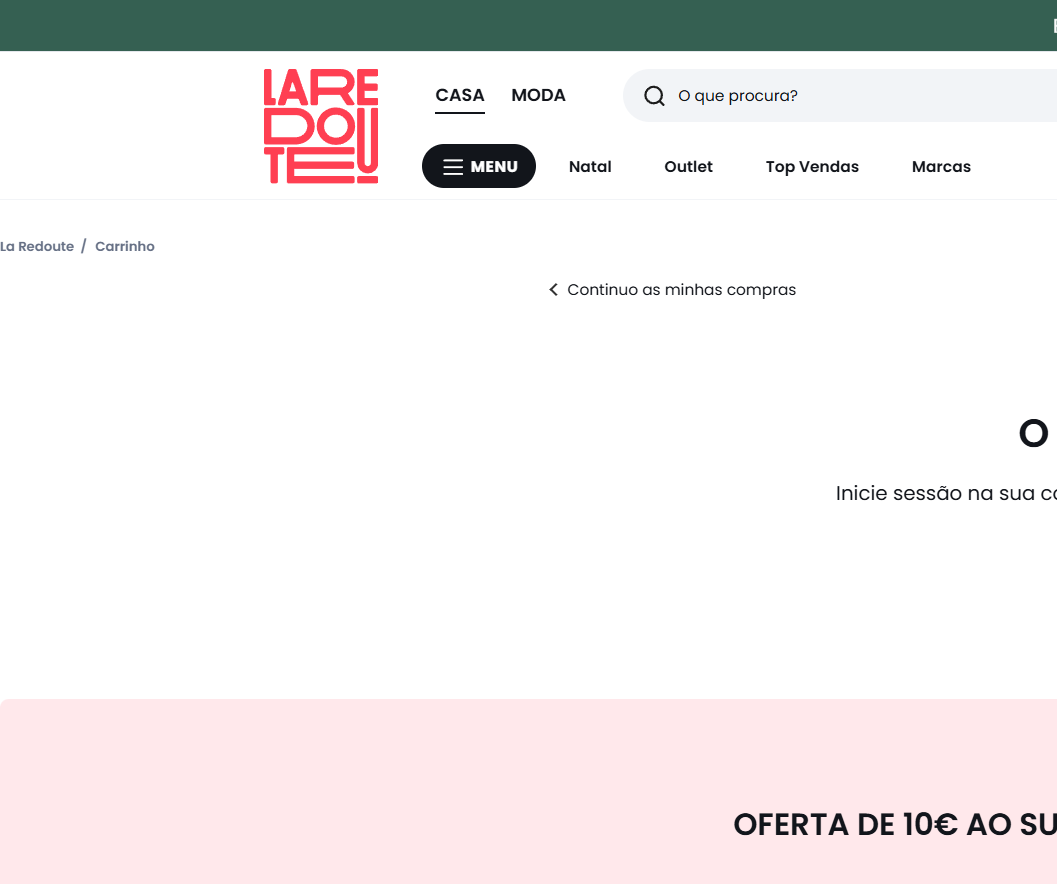
\includegraphics[width=\textwidth, keepaspectratio]{heuristics/03breadcrumbs_carrinho.png}

\newpage
    \begin{table}[h!]
        \centering
        \begin{tabular}{|m{3cm}|m{12cm}|}
        \hline
        \multicolumn{2}{|c|}{\textbf{Registo 4}} \\ \hline
        \textbf{Tarefa}       & Criar uma conta\\ \hline
        \textbf{Local}        & Ao aceder a página de Registo \\ \hline
        \textbf{Heurística}   & 5  \\ \hline
        \textbf{Descrição}    & A distinção entre particular e empresa é feita no campo de gênero. \\ \hline
        \textbf{Frequência}   & Apenas uma vez \\ \hline
        \textbf{Persistência} & Persistente \\ \hline
        \textbf{Severidade}   & 2 \\ \hline
        \textbf{Solução}      & Adicionar um novo campo de input para realizar a distinção entre particular e empresa. \\ \hline
        \end{tabular}
    \end{table}
    
    \vspace{0.5cm}
    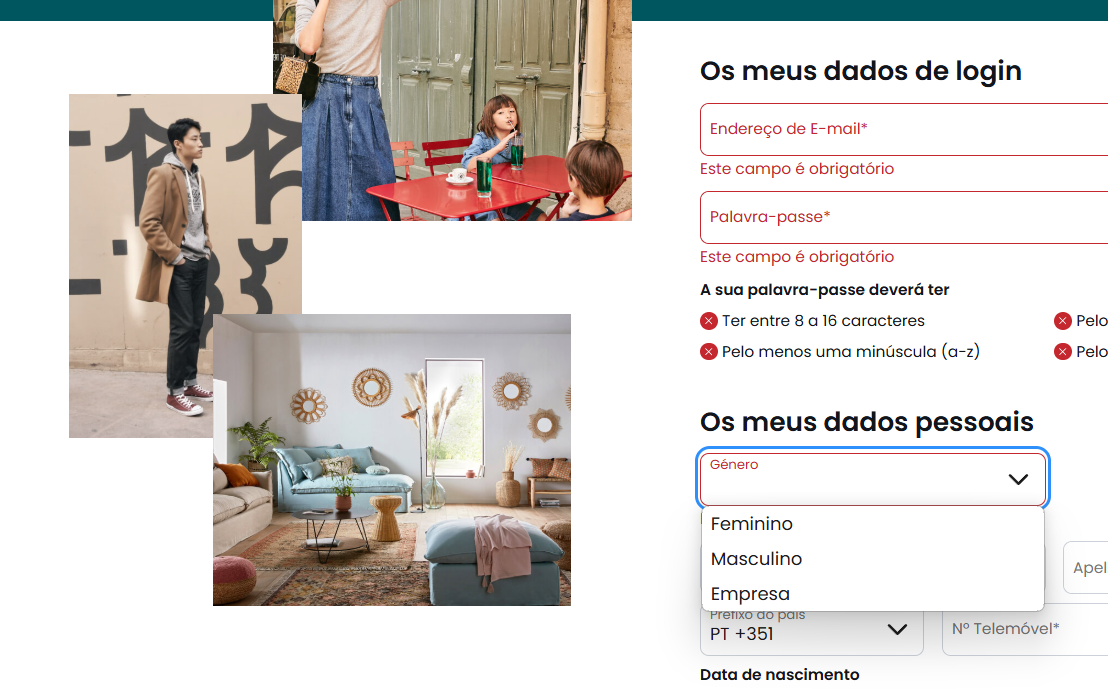
\includegraphics[width=\textwidth, keepaspectratio]{heuristics/04genero_registo.png}

    \newpage
    \begin{table}[h!]
        \centering
        \begin{tabular}{|m{3cm}|m{12cm}|}
        \hline
        \multicolumn{2}{|c|}{\textbf{Registo 5}} \\ \hline
        \textbf{Tarefa}       & Abrir a página inicial \\ \hline
        \textbf{Local}        & Página principal do website \\ \hline
        \textbf{Heurística}   & 8  \\ \hline
        \textbf{Descrição}    & O banner animado é excessivamente grande em relação à pouca informação que apresenta, ofuscando o restante conteúdo. \\ \hline
        \textbf{Frequência}   & Sempre \\ \hline
        \textbf{Persistência} & Persistente \\ \hline
        \textbf{Severidade}   & 1 \\ \hline
        \textbf{Solução}      &Reduzir o tamanho deste banner. \\ \hline
        \end{tabular}
    \end{table}
    
    \vspace{0.5cm}
    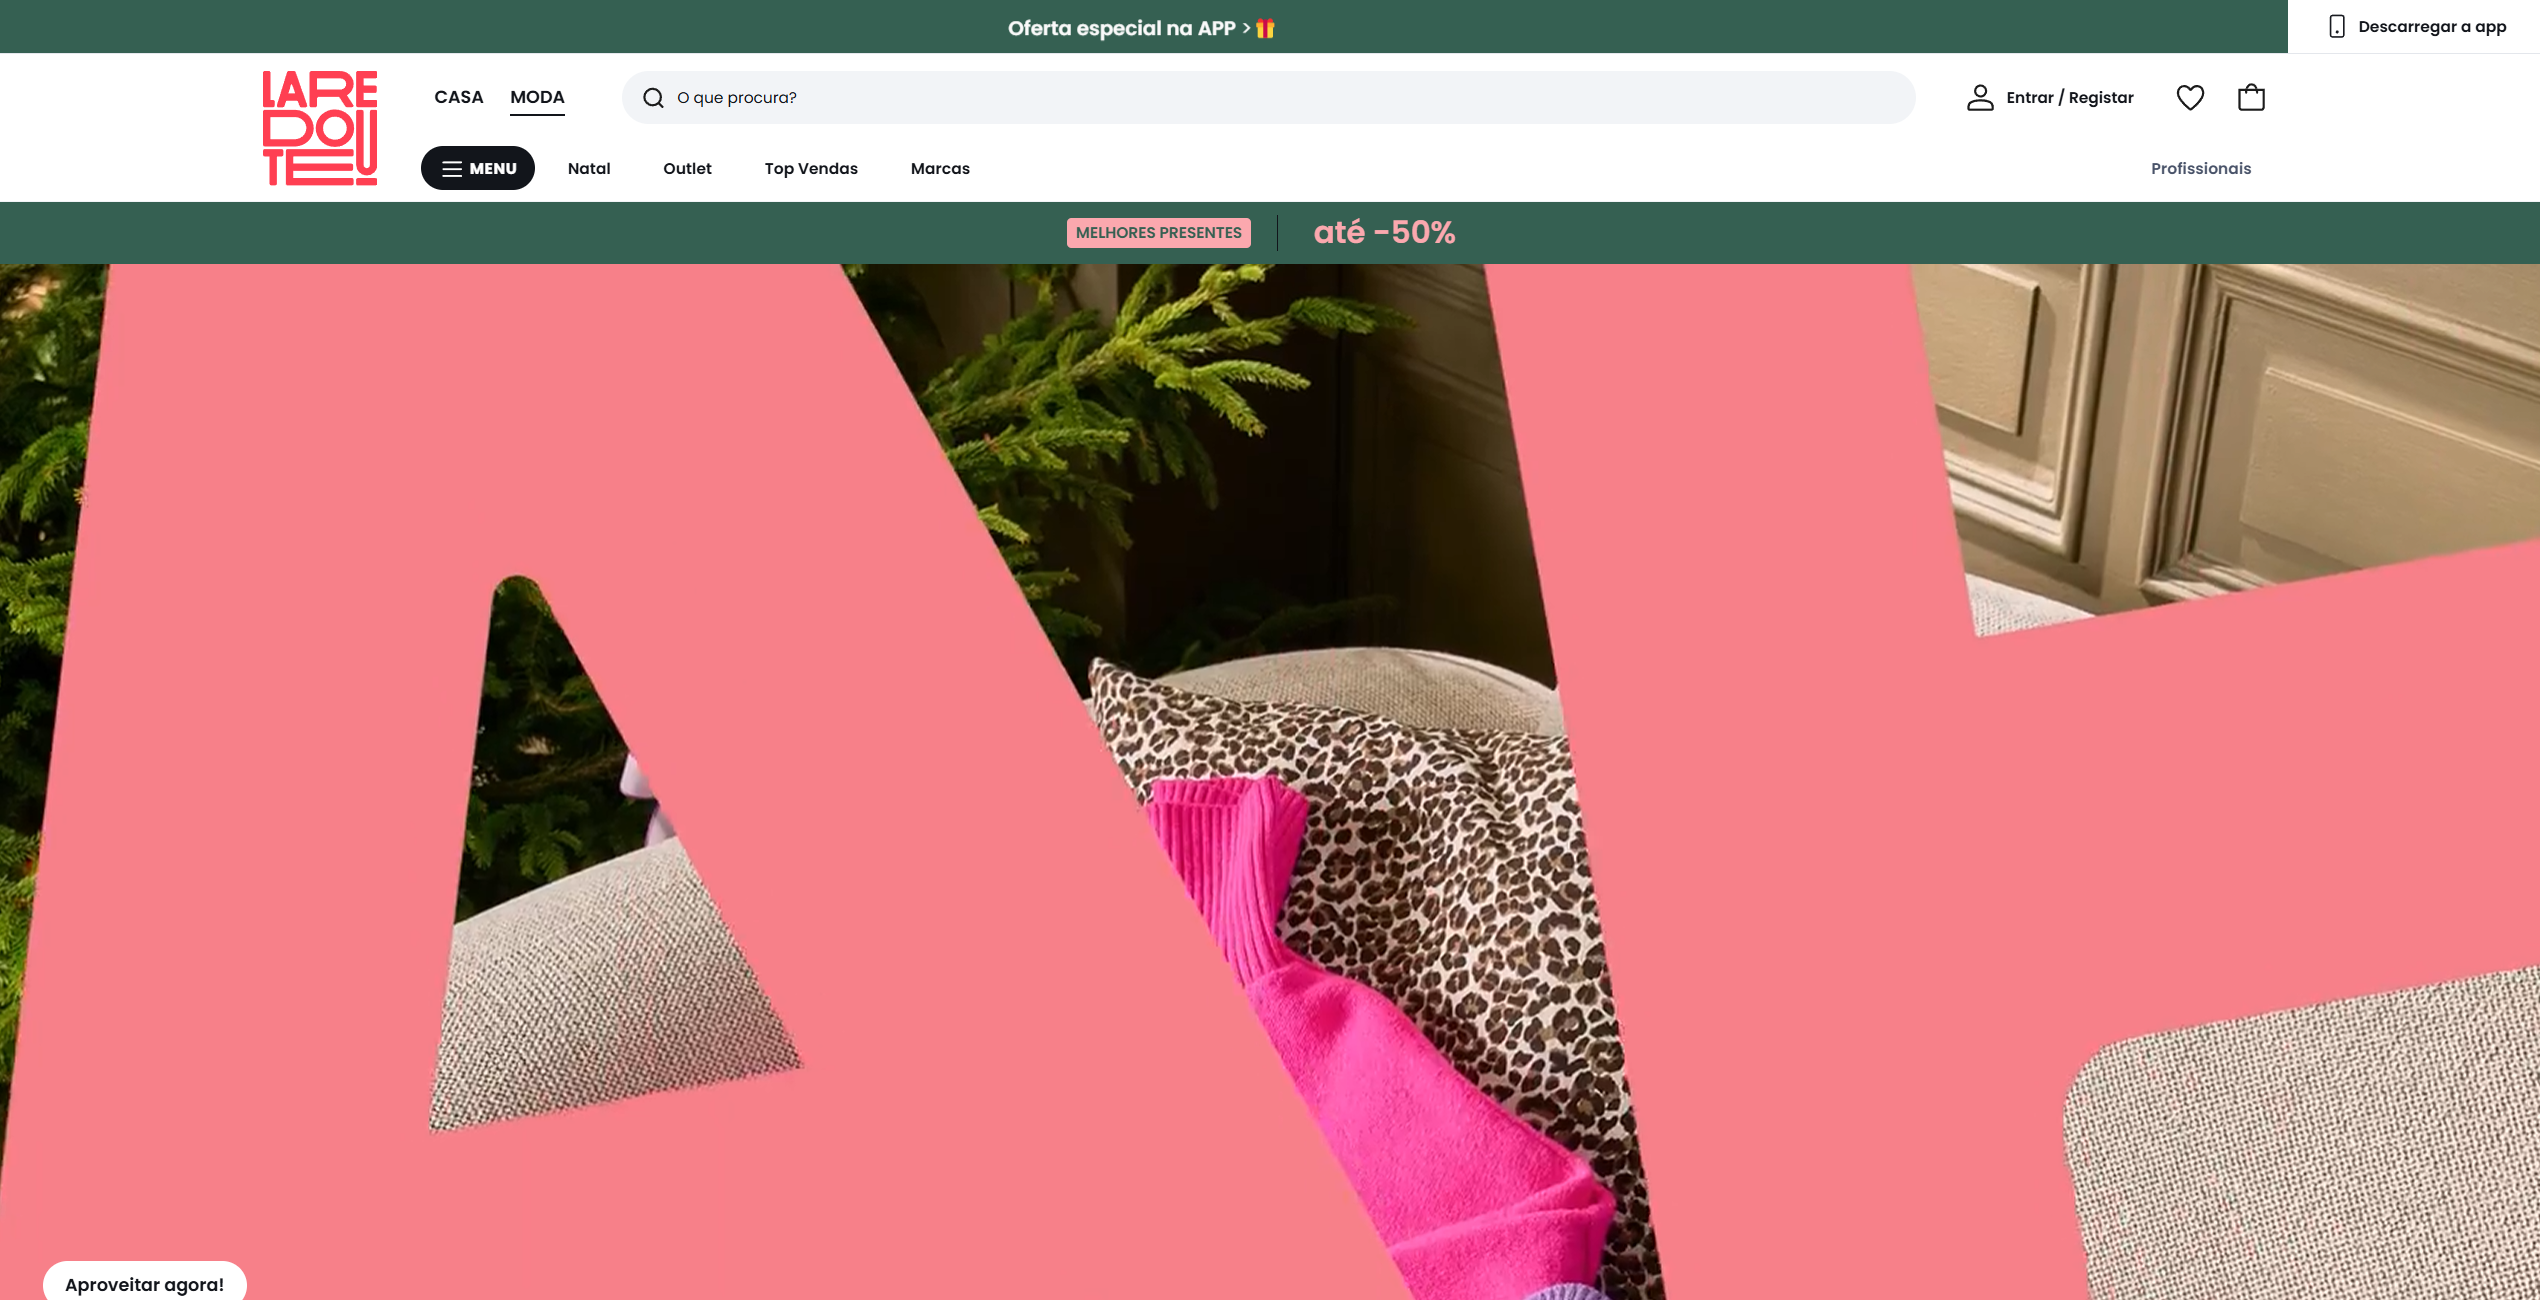
\includegraphics[width=\textwidth, keepaspectratio]{heuristics/05informacao_homepage.png}

    \newpage
    \begin{table}[h!]
        \centering
        \begin{tabular}{|m{3cm}|m{12cm}|}
        \hline
        \multicolumn{2}{|c|}{\textbf{Registo 6}} \\ \hline
        \textbf{Tarefa}       & Criação de conta \\ \hline
        \textbf{Local}        & Página de registo \\ \hline
        \textbf{Heurística}   & 3  \\ \hline
        \textbf{Descrição}    & O campo do número de telemóvel e o campo da morada não são opcionais. \\ \hline
        \textbf{Frequência}   & Sempre \\ \hline
        \textbf{Persistência} & Persistente \\ \hline
        \textbf{Severidade}   & 0 \\ \hline
        \textbf{Solução}      & Deixar estas informações como opcionais e torná-las obrigatórias apenas ao realizar a compra. \\ \hline
        \end{tabular}
    \end{table}
    
    \vspace{0.5cm}
    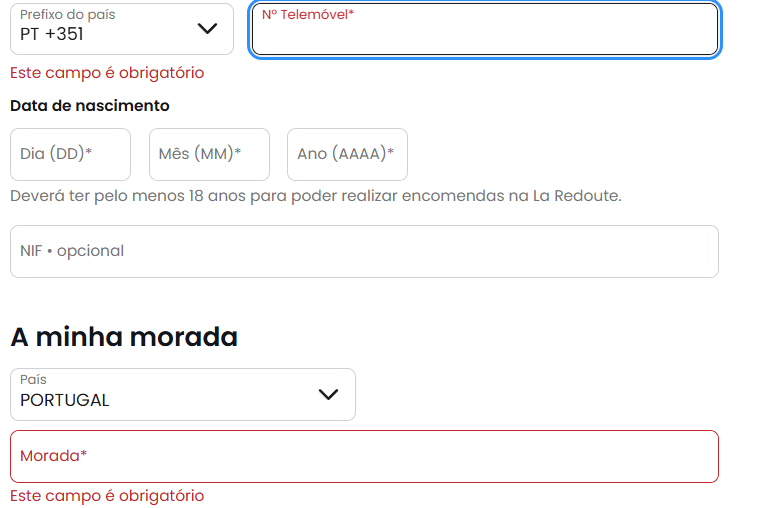
\includegraphics[width=\textwidth, keepaspectratio]{heuristics/06telefone_registo.png}

    \newpage
    \begin{table}[h!]
        \centering
        \begin{tabular}{|m{3cm}|m{12cm}|}
        \hline
        \multicolumn{2}{|c|}{\textbf{Registo 7}} \\ \hline
        \textbf{Tarefa}       & Remover um produto de carrinho \\ \hline
        \textbf{Local}        & Página do carrinho \\ \hline
        \textbf{Heurística}   & 5, 9  \\ \hline
        \textbf{Descrição}    & Não há nenhuma confirmação ao tentar remover um artigo do carrinho. \\ \hline
        \textbf{Frequência}   & Sempre \\ \hline
        \textbf{Persistência} & Persistente \\ \hline
        \textbf{Severidade}   & 2 \\ \hline
        \textbf{Solução}      & Adicionar um pop up de confirmação. \\ \hline
        \end{tabular}
    \end{table}
    
    \vspace{0.5cm}
    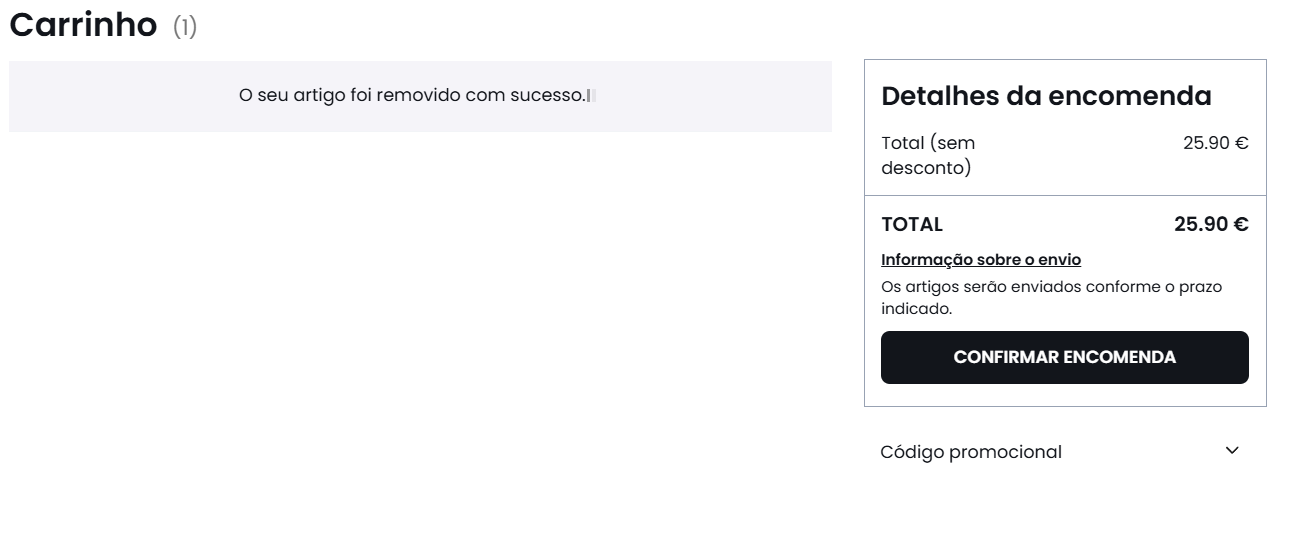
\includegraphics[width=\textwidth, keepaspectratio]{heuristics/07confirmacao_carrinho.png}

    \newpage
    \begin{table}[h!]
        \centering
        \begin{tabular}{|m{3cm}|m{12cm}|}
        \hline
        \multicolumn{2}{|c|}{\textbf{Registo 7}} \\ \hline
        \textbf{Tarefa}       & Ao efetuar o registo \\ \hline
        \textbf{Local}        & Página do registo \\ \hline
        \textbf{Heurística}   & 5, 9  \\ \hline
        \textbf{Descrição}    & Não há nenhuma validação para o código postal. \\ \hline
        \textbf{Frequência}   & Apenas uma vez \\ \hline
        \textbf{Persistência} & Persistente \\ \hline
        \textbf{Severidade}   & 3 \\ \hline
        \textbf{Solução}      & Adicionar validação a este campo. \\ \hline
        \end{tabular}
    \end{table}
    
    \vspace{0.5cm}
    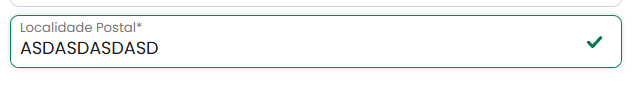
\includegraphics[width=\textwidth, keepaspectratio]{heuristics/08validacao_postal_registo.png}
\end{center}

\newpage
\section{Análise de Utilizadores e Tarefas}

\begin{center}
    \href{https://forms.gle/mGgTZJcjzfStsLvn6}{Link para o formulário}

    \vspace{0.3cm}
    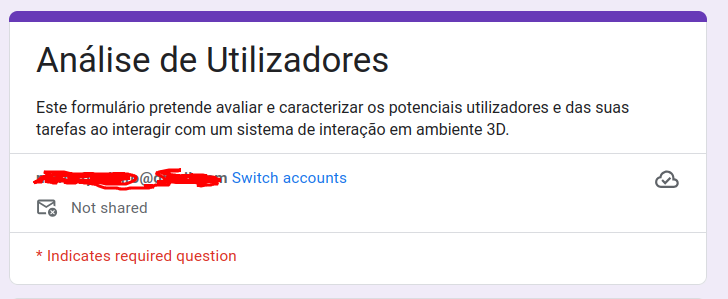
\includegraphics[width=0.75\textwidth]{form/intro_form.png}
    
\includegraphics[width=0.75\textwidth]{form/01questao_genero.png}
    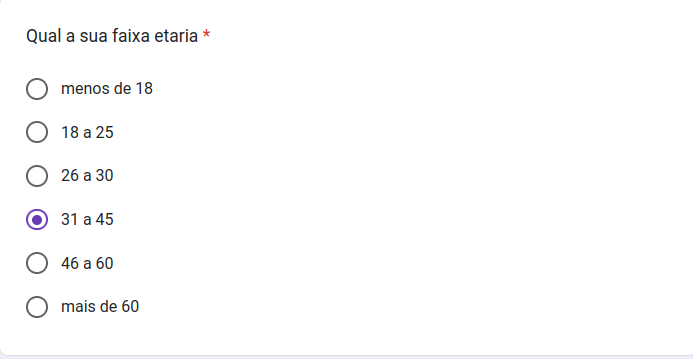
\includegraphics[width=0.75\textwidth]{form/02questao_idade.png}
    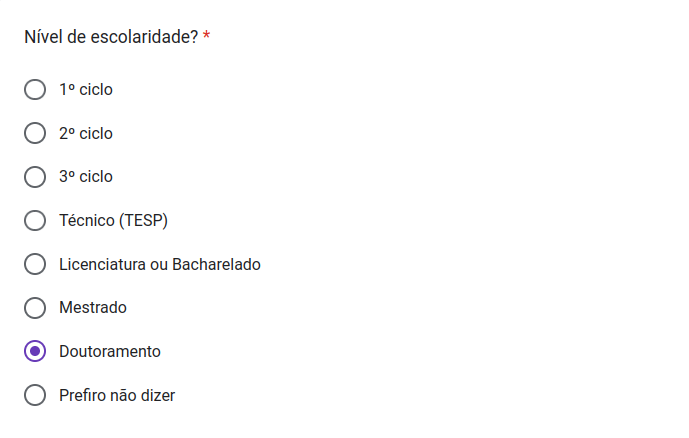
\includegraphics[width=0.75\textwidth]{form/03questao_escolaridade.png}
    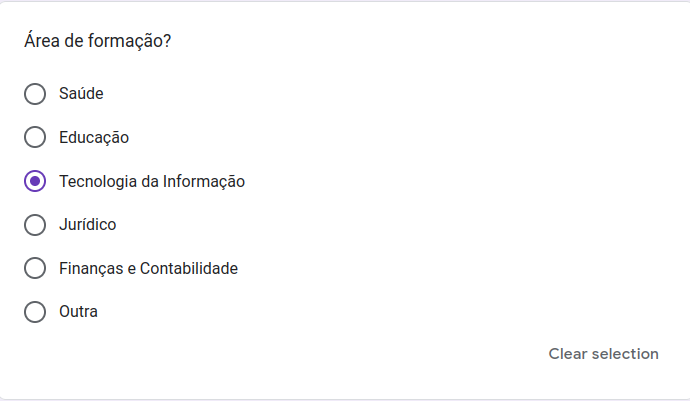
\includegraphics[width=0.75\textwidth]{form/04questao_formacao.png}
    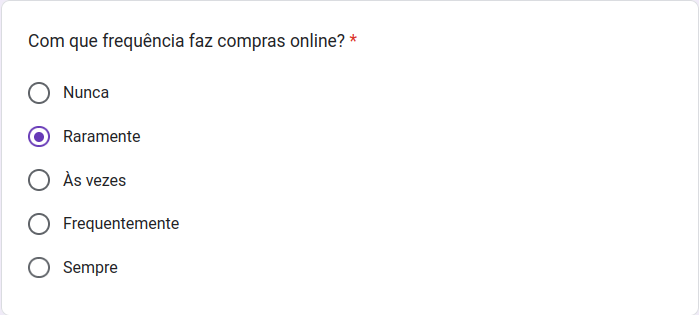
\includegraphics[width=0.75\textwidth]{form/05questao_comprasonline.png}
    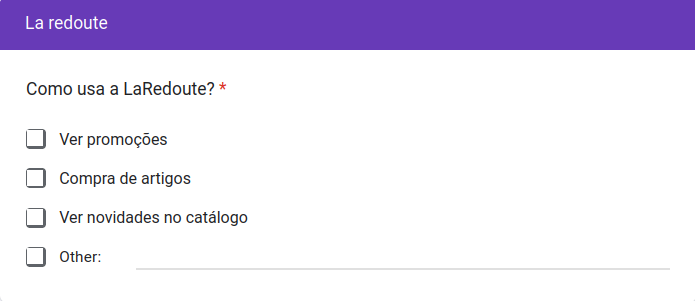
\includegraphics[width=0.75\textwidth]{form/06questao_usolaredoute.png}
    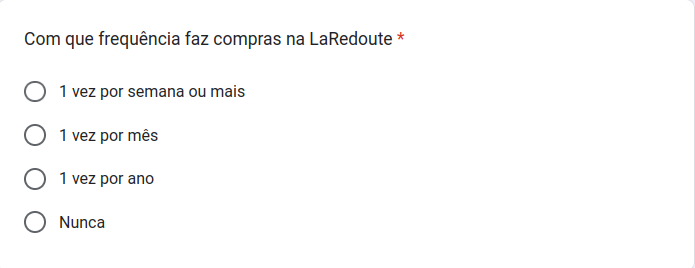
\includegraphics[width=0.75\textwidth]{form/07questao_frequencialaredoute.png}
    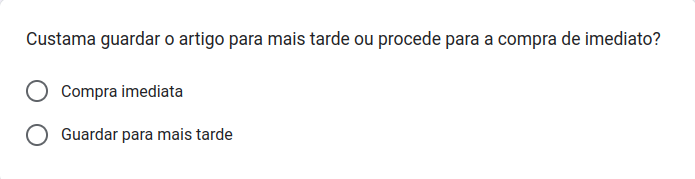
\includegraphics[width=0.75\textwidth]{form/08questao_guardarparatarde.png}
    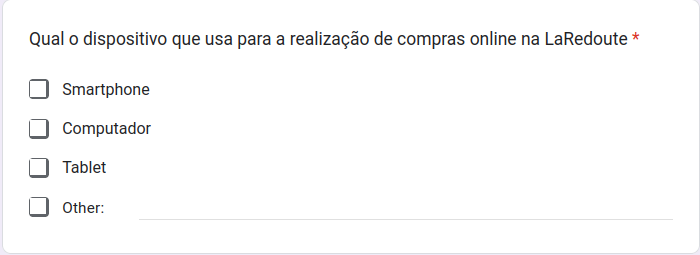
\includegraphics[width=0.75\textwidth]{form/09questao_dispositivocompra.png}
    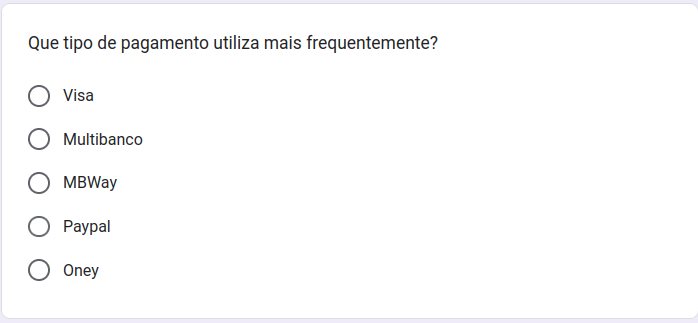
\includegraphics[width=0.75\textwidth]{form/10questao_metodopagamento.png}
    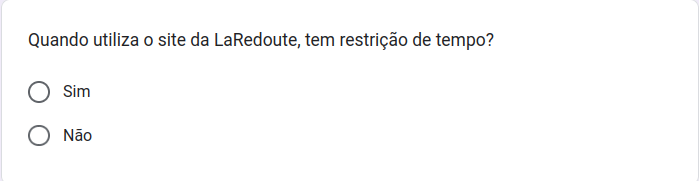
\includegraphics[width=0.75\textwidth]{form/11questao_restricaotempo.png}
    
\includegraphics[width=0.75\textwidth]{form/12questao_filtrardimensoes.png}
    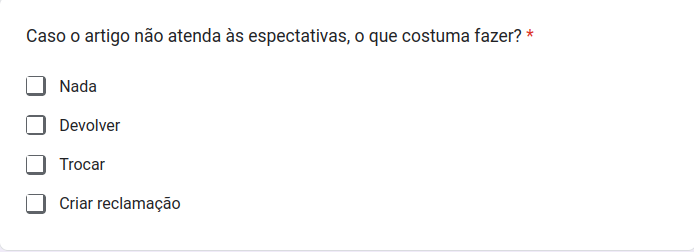
\includegraphics[width=0.75\textwidth]{form/13questao_expectativas.png}
    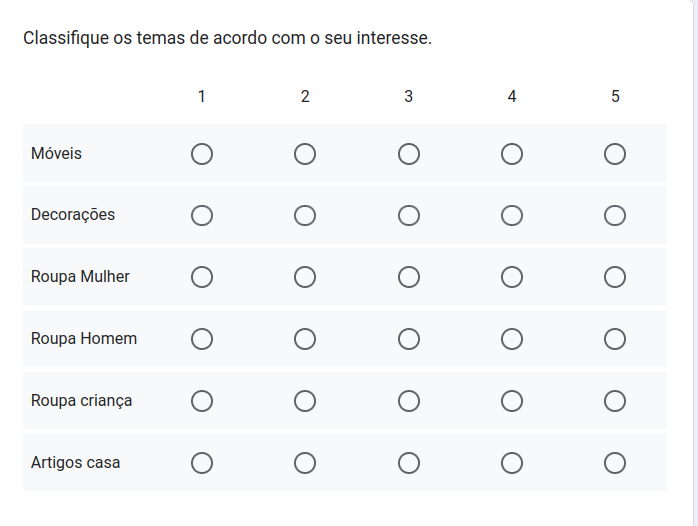
\includegraphics[width=0.75\textwidth]{form/14questao_temasinteresse.png}
    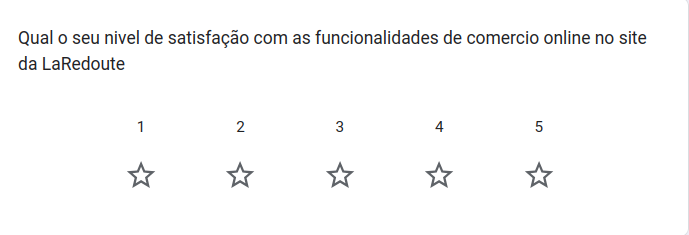
\includegraphics[width=0.75\textwidth]{form/15questao_satisfacao.png}
    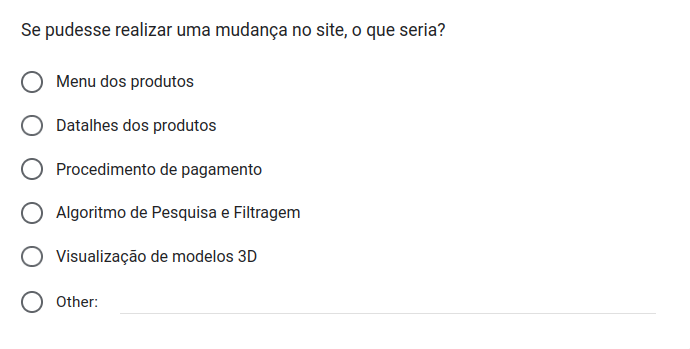
\includegraphics[width=0.75\textwidth]{form/16questao_mudancasite.png}
    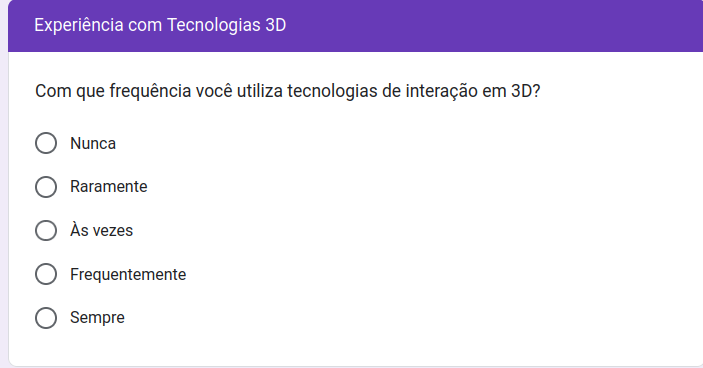
\includegraphics[width=0.75\textwidth]{form/17questao_frequencia3d.png}
    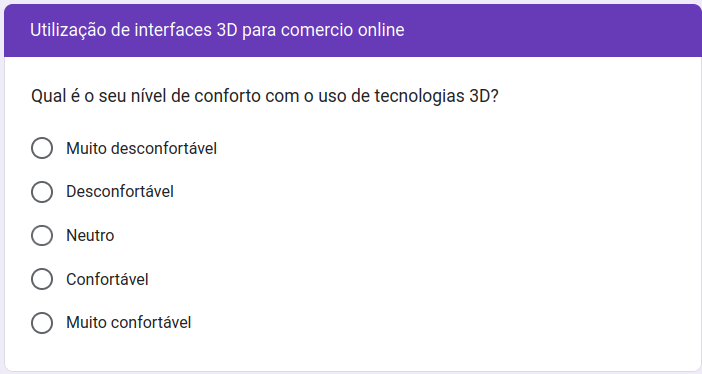
\includegraphics[width=0.75\textwidth]{form/18questao_conforto3d.png}
    
\includegraphics[width=0.75\textwidth]{form/19questao_visao3d.png}
    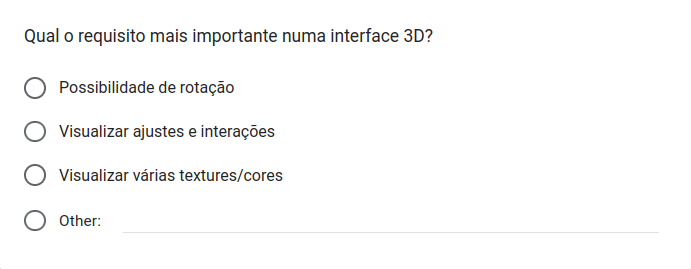
\includegraphics[width=0.75\textwidth]{form/20questao_requisito3d.png}
\end{center}

\newpage
\section{Requisitos funcionais}
    Permitir que o utilizador possa:
    \begin{itemize}
        \item Escolher diferentes textures
        \item Efetuar rotações ao objeto 3D
        \item Visualizar uma animação que muda o ângulo do braço do candeeiro
    \end{itemize}

\newpage
\section{Avaliação da Usabilidade do Sistema}

\newpage
\section{Análise/Discussão dos resultados}


\end{document}
